\section{Аналитический раздел}

\subsection{Постановка задачи}

В соответствии с техническим заданием, требуется написать драйвер геймпада Logitech F310 для использования его в качестве мыши и клавиатуры.

Для решения поставленной задачи необходимо:

\begin{itemize}[leftmargin=1.6\parindent]
    \item[---] проанализировать особенности работы геймпада,
    \item[---] рассмотреть способы получения данных от устройства с использованием подсистемы USB,
    \item[---] исследовать подсистему ввода для интерактивных устройств,
    \item[---] разработать драйвер в виде загружаемого модуля ядра,
    \item[---] провести исследование разработанного драйвера.
\end{itemize}

\subsection{Анализ особенностей работы геймпада}

Устройство геймпада Logitech F310 приведено на рисунке \ref{fig:gamepad}.

\begin{figure}[ht]
    \centering
    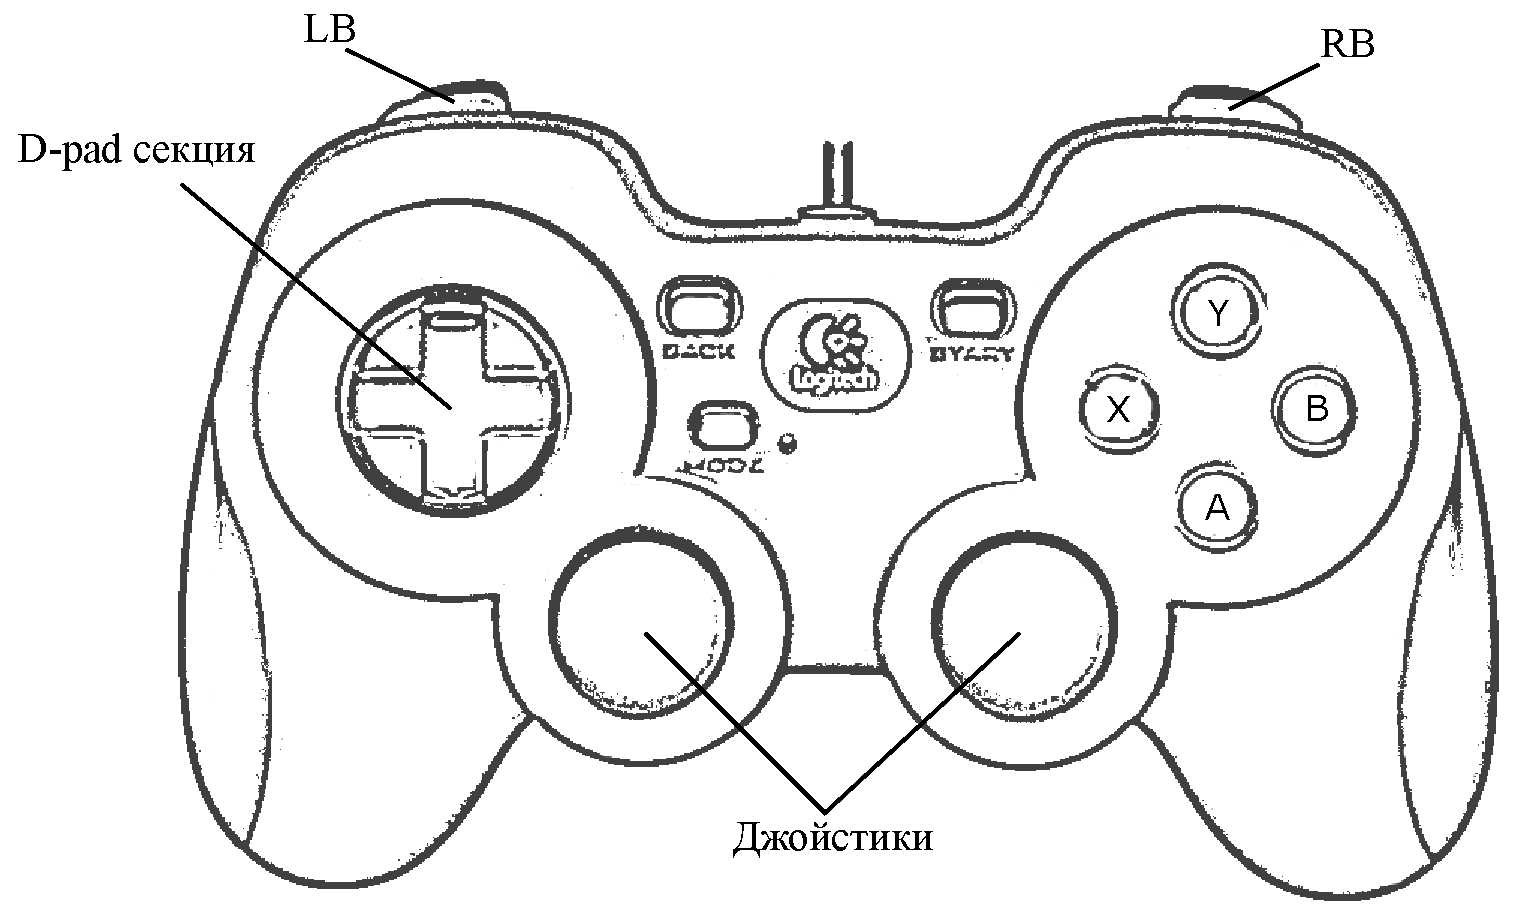
\includegraphics[width=0.9\linewidth]{img/gamepad.pdf}
    \caption{Геймпад Logitech F310}
    \label{fig:gamepad}
\end{figure}

В составе геймпада имеются два джойстика, положение которых кодируется двумя независимыми парами величин -- смещениями вдоль горизонтальной и вертикальной осей соответственно (рисунок \ref{fig:gamepad:axes}). Смещение может принимать целочисленные значения в интервале от -127 до 128.

\begin{figure}[ht]
    \centering
    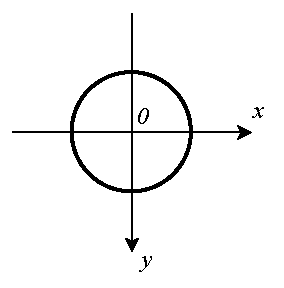
\includegraphics[width=0.4\linewidth]{img/joystick_axes.pdf}
    \caption{Система координат джойстика}
    \label{fig:gamepad:axes}
\end{figure}

Так как геймпад Logitech F310 подключается по USB, при написании драйвера будет использована подсистема USB.

\subsection{Подсистема USB}

% === ПРО HID ЛУЧШЕ НЕ ПИСАТЬ ПОТОМУ ЧТО ЭТО ВЫХОДИТ ОПТИМАЛЬНЕЕ ЧЕМ ОБЫЧНЫЙ USB ДРАЙВЕР. И ЗАЧЕМ Я ТОГДА ПАРИЛСЯ??? НЕПОНЯТНО ===
%В операционной системе Linux существует несколько вариантов регистрации драйвера для USB устройства:

%\begin{itemize}[leftmargin=1.6\parindent]
%    \item[---] регистрация HID драйвера,
%    \item[---] регистрация USB драйвера.
%\end{itemize}

% При регистрации HID драйвера ...

% === ОПИШЕМ В ОБЩЕМ ВИДЕ РЕГИСТРАЦИЮ USB ДРАЙВЕРА

USB драйвер имеет две точки входа -- \texttt{probe} и \texttt{disconnect}, которые вызываются подсистемой USB при подключении и отключении устройства, соответствующего данному драйверу.

Обмен информацией между подключенным устройством и драйвером осуществляется пакетами по запросу. Блок запроса USB (USB Request Block -- URB) представляется структурой ядра \texttt{urb}:

\begin{small}
\begin{verbatim}
struct urb {
    struct list_head urb_list;
    struct usb_device *dev; /* (in) pointer to associated device */
    unsigned int pipe; /* (in) pipe information */
    int status; /* (return) non-ISO status */
    void *transfer_buffer; /* (in) associated data buffer */
    dma_addr_t transfer_dma; /* (in) dma addr for transfer_buffer */
    u32 transfer_buffer_length; /* (in) data buffer length */
    u32 actual_length; /* (return) actual transfer length */
    int interval; /* (modify) transfer interval */
    void *context; /* (in) context for completion */
    usb_complete_t complete; /* (in) completion routine */
    /* ... */
};
\end{verbatim}
\end{small}

\subsubsection{Способы передачи URB пакетов}

Передача URB пакетов по шине USB является дуплексной и может происходить в одной из четырех форм, в зависимости от подключенного устройства:

\begin{itemize}[leftmargin=1.6\parindent]
    \item[---] \texttt{Control} -- используется для передачи управляющих команд для настройки устройства или получения его статуса.
    \item[---] \texttt{Bulk} -- используется для обмена большими пакетами данных. Зачастую именно эта форма передачи используется устройствами на подобие сканеров и SCSI адаптеров.
    \item[---] \texttt{Interrupt} -- используется для запроса передачи небольших пакетов в режиме опроса устройства. Если был запрошен пакет в режиме прерывания, то драйвер хост-контроллера автоматически будет повторять этот запрос с определенным интервалом (1--255 мс).
    \item[---] \texttt{Isochronous} -- используется для передачи данных в реальном времени с гарантированной пропускной способностью шины, но ненадежно. В общем случае изохронный тип используется для передачи аудио и видео информации. 
\end{itemize}

Так как рассматриваемое устройство -- геймпад -- является HID устройством, и поддерживает формат передачи \texttt{Interrupt}, то при реализации драйвера будет использован именно этот формат.

\subsection{Подсистема ввода для интерактивных устройств}

Подсистема ввода для интерактивных устройств представляет уровень абстракции между устройствами ввода и обработчиками ввода. Устройства ввода фиксируют входные данные от действий пользователя и генерируют входные события, которые, проходя через подсистему ввода, отправляются соответствующим обработчикам. Ядро ввода обеспечивает сопоставление "многие ко многим"\, между устройствами ввода и обработчиками событий.

Список наиболее распространенных типов событий, генерируемых с использованием данной подсистемы:

\begin{itemize}[leftmargin=1.6\parindent]
    \item[---] \texttt{EV\_KEY} -- используется для описания изменений состояния клавиатур, кнопок или других устройств, похожих на клавиши;
    \item[---] \texttt{EV\_REL} -- используется для описания изменения значения относительной оси, например, перемещения мыши на 5 единиц влево;
    \item[---] \texttt{EV\_ABS} -- используется для описания изменений значений абсолютной оси, например, описания координат касания на сенсорном экране.
\end{itemize}

\subsubsection{Использование геймпада в качестве мыши}

Для реализации управления мышью через геймпад предложено использование джойстиков (один для перемещения мыши, второй для управления колесиком мыши). Кнопки геймпада A и B предложено назначить на кнопки мыши (левую и правую соответственно).

Изменение положения курсора на экране происходит посредством генерирования события типа \texttt{EV\_REL}. Согласно спецификации геймпада \cite{gamepad-spec}, движение джойстиков генерирует события типа \texttt{EV\_ABS}. В связи с этим, реализация движения курсора будет некорректной при простой замене одного типа события на другой -- фиксация джойстика в смещенном положении не будет приводить к поступлению новых URB пакетов и генерированию новых событий перемещения мыши, и как следствие не будет происходить изменение положения курсора.

Для решения изложенной проблемы необходимо использовать таймер, который должен с постоянной периодичностью генерировать события при возникновении описанной ситуации. Для работы с таймером в ядре существует структура \texttt{timer\_list}.

\begin{small}
\begin{verbatim}
struct timer_list {
    struct hlist_node entry;
    unsigned long expires;
    void (*function)(struct timer_list *);
    u32	flags;
};

#define timer_setup(timer, callback, flags) /* ... */
int del_timer(struct timer_list *timer);
\end{verbatim}
\end{small}

Запуск таймера должен происходить только тогда, когда джойстики находятся в смещенном положении. Планирование следующего выполнения осуществляется вызовом функции \texttt{mod\_timer}.

\begin{small}
\begin{verbatim}
#define TIMER_PERIOD (HZ / 100) // 10 ms
mod_timer(&timer, jiffies + TIMER_PERIOD);
\end{verbatim}
\end{small}

\subsubsection{Использование геймпада в качестве клавиатуры}

Ввод символов является задачей не свойственной геймпаду -- количество имеющихся кнопок на устройстве не позволяет установить их однозначного соответствия символам, вводимым с клавиатуры.

В качестве решения данной задачи предложено использование виртуальной клавиатуры (рисунок \ref{fig:virtual-kbd}) и указателя, перемещение которого осуществляется с использованием D-pad секции на геймпаде (рисунок \ref{fig:gamepad}). Ввод символа под указателем осуществляется нажатием кнопки LB на геймпаде. Таким образом можно вводить любой символ, располагающийся на виртуальной клавиатуре.

\begin{figure}[ht]
    \centering
    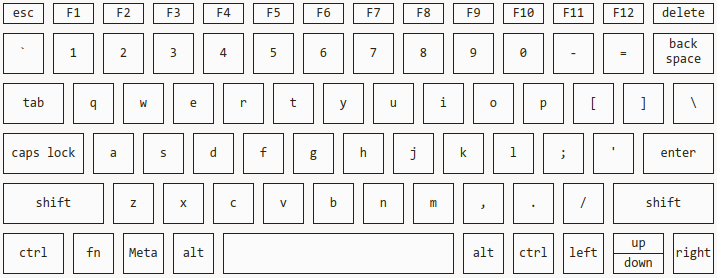
\includegraphics[width=\linewidth]{img/virtual_keyboard_white.png}
    \caption{Виртуальная клавиатура}
    \label{fig:virtual-kbd}
\end{figure}

Однако для отслеживания позиции указателя нужно иметь возможность отобразить на экране виртуальную клавиатуру вместе с текущей позицией указателя. Так как работа с дисплеем напрямую из ядра требует учета множества факторов, управление отображением виртуальной клавиатуры напрямую из ядра становится трудоемкой задачей.

Более оптимальным вариантом является написание демона, который по запросу будет выводить на экран виртуальную клавиатуру.

\subsection{Взаимодействие драйвера и демона}

Одним из возможных способов передачи информации из пространства ядра в пространство пользователя является использование виртуальной файловой системы proc \cite{vfs-proc}.

Операции, которые могут быть осуществлены с файлом определяются структурой \texttt{proc\_ops}. В случае реализации передачи событий из пространства ядра в пространство пользователя, необходимо и достаточно реализовать две операции: \texttt{open} и \texttt{read}.

При этом, если события не возникают, процесс должен быть заблокирован при попытке чтения. Необходимость блокировки процесса и ожидания появления нового события приводит к использованию очередей ожидания, которые представляются в ядре структурой \texttt{wait\_queue\_head}:

\begin{small}
\begin{verbatim}
struct wait_queue_entry {
    unsigned int flags;
    void *private;
    wait_queue_func_t func;
    struct list_head entry;
};

struct wait_queue_head {
    spinlock_t lock;
    struct list_head head;
};
\end{verbatim}
\end{small}

Блокировка процесса и ожидание возникновения события осуществляется вызовом макроса

\texttt{wait\_event\_interruptible(wq\_head, condition)}.

Все ждущие в данной очереди процессы пробуждаются посредством вызова макроса \texttt{wake\_up\_all(wq\_head)}, после чего будет анализировано выражение \texttt{condition} переданное при блокировке. Если оно ложно, то процесс вновь блокируется.

\subsection*{Выводы}

Использование геймпада в качестве мыши и клавиатуры имеет ряд особенностей:

\begin{enumerate}[leftmargin=1.6\parindent]
    \item тип событий, генерируемых геймпадом по спецификации не совместим с типом события перемещения мыши -- реализация перемещения мыши требует использования таймеров;
    \item непосредственное сопоставление скан-кодов клавиш на клавиатуре с кнопками геймпада невозможно -- необходима реализация поддержки виртуальной клавиатуры.
\end{enumerate}

\pagebreak
